\documentclass[12pt]{article} % 

\usepackage[hyperfootnotes=false]{hyperref}
\usepackage[margin=1.2in]{geometry}                                      
\usepackage{amsmath,amsthm,amssymb} 
\usepackage{titlesec}                                                   
\usepackage{bm}
\usepackage{cprotect}
\usepackage[all=normal, title=tight]{savetrees}
\usepackage{bbold}
\usepackage{abstract}
                                           
\usepackage{graphicx}                                                          
\graphicspath{{../data/}}

\usepackage{biblatex}
\bibliography{bib.bib}

\usepackage{tikz}
\usetikzlibrary{arrows,shapes,trees,backgrounds} 
\definecolor{mygray}{gray}{.4}

\usepackage{listings}
\lstset{basicstyle=\ttfamily,breaklines=true}

%%%%%%%%%%%%%%%%%%%%%%%%%%%%%%%%%%%%%%%%%%%%%%%%%%%%%%%
% Taken from Kitaev Unpaired fermions...
\newenvironment{subfig}[1]%
{\def\subfigLabel{#1}\begin{tabular}[b]{@{}c@{}}}%
	{\\[10pt]\subfigLabel\end{tabular}}

\newsavebox{\TempBox}
\newlength{\TempLength}
%%%%%%%%%%%%%%%%%%%%%%%%%%%%%%%%%%%%%%%%%%%%%%%%%%%%%%%

       

\titleformat{\subsection}[runin]
{\normalfont\large\bfseries}{\thesubsection}{1em}{}

\renewcommand{\bf}{\mathbf}
\renewcommand{\cal}{\mathcal}
\newcommand{\pd}[2]{\frac{\partial #1}{\partial #2}}
\newcommand{\pdn}[3]{\frac{\partial^{#3} #1}{\partial #2^{#3}}}
\newcommand{\pdop}[1]{\frac{\partial}{\partial #1}}
\newcommand{\nd}[2]{\frac{d #1}{d #2}}
\newcommand{\ndn}[3]{\frac{d^{#3} #1}{d #2^{#3}}}
\newcommand{\ndop}[1]{\frac{d}{d #1}}
\newcommand{\dt}{\frac{d}{dt}}
\newcommand{\grad}{\bm\nabla}
\newcommand{\cross}{\times}
\newcommand{\curl}{\grad\cross}
\newcommand{\imp}{\Longrightarrow\quad}
\newcommand{\abs}[1]{\left|#1\right|}
\newcommand{\half}{\frac{1}{2}}
\newcommand{\third}{\frac{1}{3}}
\renewcommand{\th}[1]{\frac{1}{#1}}
\renewcommand{\k}{4\pi\epsilon_0}
\newcommand{\eps}{\epsilon_0}
\newcommand{\intt}{\int_{t_1}^{t_2}}
\newcommand{\inti}{\int_{-\infty}^{+\infty}}
\newcommand{\ex}[1]{\left\langle #1 \right\rangle}
\renewcommand{\d}{\delta}
\newcommand{\e}{\text{e}}
\renewcommand{\l}{\ell}
\newcommand{\om}{\omega}
\newcommand{\h}{\hbar}
\newcommand{\ket}[1]{\left|#1\right\rangle}
\newcommand{\bra}[1]{\left\langle#1\right|}
\newcommand{\braket}[2]{\left\langle#1\middle|#2\right\rangle}
\newcommand{\brakett}[3]{\left\langle#1\middle|#2\middle|#3\right\rangle}
\newcommand{\comm}[2]{\left[#1,#2\right]}
\newcommand{\acom}[2]{\left\{#1,#2\right\}}
\newcommand{\nn}{\nonumber\\}

\DeclareMathOperator{\Tr}{Tr}

%\renewcommand{\thesection}{\arabic{section}}

\begin{document}
	
\newgeometry{left=1in, right=1in, top=.5in, bottom=.8in}

\title{\textbf{Ground States and Entropy of the Supersymmetric SYK Model}}
\author{Charles Stahl\footnote{I pledge my honor that this paper represents my own work in accordance with University regulations.}\\
		Advised by Prof. Herman Verlinde}

\maketitle

\begin{abstract}
	This paper explores the ground states of a supersymmetric generalization of the Sachdev-Ye-Kitaev model, with $N$ interacting Majorana fermions. The model consists of all-to-all interactions between $N$ Majorana fermions, mediated by a Hamiltonian that connects fermions in groups of 4. The supersymmetric model defines a supercharge that connects 3 fermions, with the Hamiltonian being the square of the supercharge. The number of ground states is large and extensive in this model, leading to extensive entropy. Numerical simulations of the number of ground states and entropy confirm these features for small $N$. 
\end{abstract}

\tableofcontents
\newpage
\restoregeometry

\section{Introduction} \label{sec:intro}

The Sachdev-Ye-Kitaev (SYK) model is a model of random uncorrelated interactions between $N$ fermions. Sachdev and Ye introduced a model in 1993 with pairwise interactions in~\cite{sachdev93}. In~\cite{kitaev15} Kitaev generalized the model to interactions between 4 fermions, with Hamiltonian
\begin{align}
H = \sum_{ijkl}J_{ijkl}\psi_i\psi_j\psi_k\psi_l.
\end{align} 
In general, the models can have terms in the Hamiltonian connecting $\hat{q}$ fermions with $\hat{q}$ even. 

The holographic connection of this model to black holes with Andi-de Sitter (AdS) horizons was discussed by Sachdev in 2010~\cite{sachdev10}. The model is maximally chaotic~\cite{kitaev00}. The infinite range any-to-any interactions lead to non-zero entropy even at $T=0$. This has been confirmed for large $N$ numerically~\cite{Georges2001}. The extensive entropy is associated with the horizon of an extremal black hole in Anti-de Sitter space (AdS/CFT correspondence)~\cite{fu16}. This paper does not include discussion of the AdS/CFT correspondence, but an extensive introduction can be found in \cite{Aharony2000}. For more background on the SYK model see~\cite{mald16}.

The model is built of Majorana fermions, which are fermions that are their own antiparticles~\cite{elliott14}. Dirac fermions are solutions to the Dirac equation
\begin{align}
(\gamma^\mu\partial_\mu - m)\Phi = 0,
\end{align}
which are 4-component spinors. Two degrees of freedom are due to the choice of helicity, while the other two differentiate fermions from antifermions. 

The Majorana basis allows the equation to be separated into two coupled systems. Each of these is then a Majorana fermion. Since they do not evolve independently, the Majorana basis does not simplify the description of Dirac fermions. The basis would, however, simplify the description of unpaired Majorana fermions. 

No fundamental particles are known to be Majorana fermions, but the status of neutrinos is unknown currently. If neutrinoless double decay occurs, then neutrinos must be Majorana~\cite{elliott14}. The standard model does not include Majorana neutrinos. The Majorana algebra can however describe emergent quasiparticles in solid-state physics. Since the electron is a Dirac fermion, it is equivalently two coupled Majorana fermions. If these can be separated, the resultant quasiparticles are Majorana fermions. One way of doing this is on a one dimensional quantum ``wire." Dirac fermions are separated and each Majorana is paired with one from the adjacent electron. See figure~\ref{fig:pairs} for a graphical description. This process is described in detail in~\cite{kitaev00}.
\begin{figure}[ht]

\sbox{\TempBox}{
\begin{picture}(0,0)(0,0)
\put(0,0){\oval(32,16)}
\put(-10,0){\circle*{4}}
\put(10,0){\circle*{4}}
\end{picture}}
	
\newcommand\fsite[2]{
\begin{picture}(0,0)(8,0)
\put(0,0){\usebox{\TempBox}}
\put(-15,12){\footnotesize #1}
\put(15,12){\footnotesize #2}
\end{picture}}

\centering
\hbox to \textwidth {
%\hspace{.1\textwidth}

%\begin{subfig}{a}
%	\begin{picture}(100,30)(0,0)
%	\put(0, 0){\fsite{$c_1$}{$c_2$}}
%	\put(-10 ,0){\thicklines\line(1,0){20}}
%	\put(0, 0){\circle*{4}}
%	\end{picture}
%\end{subfig}
	
\begin{subfig}{a)}
\begin{picture}(170,30)(0,-8)
\put(18,0){\fsite{$c_1$}{$c_2$}}
\put(8,0){\thicklines\line(1,0){20}}
\put(75,0){\fsite{$c_3$}{$c_4$}}
\put(65,0){\thicklines\line(1,0){20}}
\put(104,0){\ldots}
\put(146,0){\fsite{$c_{2L-1}$}{$c_{2L}$}}
\put(136,0){\thicklines\line(1,0){20}}
\end{picture}
\end{subfig}
		
%\hspace{.05\textwidth}
		
\begin{subfig}{b)}
\begin{picture}(170,30)(0,-8)
\put(18,0){\fsite{$c_1$}{$c_2$}}
\put(28,0){\thicklines\line(1,0){37}}
\put(75,0){\fsite{$c_3$}{$c_4$}}
\put(85,0){\thicklines\line(1,0){18}}
\put(104,0){\ldots}
\put(146,0){\fsite{$c_{2L-1}$}{$c_{2L}$}}
\put(136,0){\thicklines\line(-1,0){18}}
\end{picture}
\end{subfig}		
}
	
\caption{\textbf{Separating Dirac fermions into Majorana fermions.}  The ovals show the physical particles, while the lines show pairings. In a) there are no unpaired Majorana fermions, but in b) both $c_1$ and $c_{2L}$ are unpaired. Image generated using code from~\cite{kitaev00}.}
\label{fig:pairs}
\end{figure}

This paper analyzes a supersymmetric generalization of the SYK model introduced in~\cite{fu16}, confirming predictions of the degeneracy of the ground state and the existence of entropy at $T=0$. Specifically it finds for a lower bound $D_\text{GS}\ge N\log\sqrt{3}$ on the number of ground states and entropy that also scales with $N$.

In section~\ref{sec:osc} I introduce second quantization and the Majorana algebra through harmonic oscillators. This is also a convenient way to introduce supersymmetry. In section~\ref{sec:syk} I define the SYK model and its supersymmetric generalizations, using the algebras defined in the previous section. In section~\ref{sec:N2gs_ent} I present calculations of ground state degeneracy and entropy, and section~\ref{sec:numeric} includes numeric calculations of these values, confirming the analytic calculations.


\section{Supersymmetry and Oscillators} \label{sec:osc}

One starting point for discussing supersymmetry is through the formalism of harmonic oscillators for bosons and fermions. The standard harmonic oscillator is easily generalized to second quantized bosonic and fermionic oscillators, from which Majorana fermions and supersymmetric oscillators can be introduced. This also allows for the introduction of the commutation and anticommutation relations for bosons and fermions. 

\subsection{Bosonic and Fermionic Oscillators} \emph{} \label{sub:bf_osc}

Consider a single harmonic oscillator 
\begin{align}
H = p^2 +\frac{\om^2 x^2}{4},\quad \comm{x}{p} = i, \label{eqn:harmosc}
\end{align}
with raising and lowering operators
\begin{align}
a = \frac{\sqrt{\om}x}{2}+\frac{i}{\sqrt{\om}}p,\quad a^\dag = \frac{\sqrt{\om 
	}x}{2}-\frac{i}{\sqrt{\om}}p,\quad \comm{a}{a^\dag } = 1. \label{eqn:bosops}
\end{align}
The Hamiltonian can then be written as 
\begin{align}
H = \om a^\dag a + \frac{\om}{2} \equiv \om \left(N + \th{2}\right).
\end{align}
After introducing a ground state $\ket{0}$ such that $a\ket{0} = 0$, the number operator $N$ counts the number of times the raising operator has been applied to a state. This shows that the raising and lowering operators add and remove energy from the system, respectively. 

It is now straightforward to introduce second quantization of bosons through an example, electromagnetism. This presentation follows~\cite{gottfried03}. Given a collection of modes $k$ with frequencies $\om_k$, the Hamiltonian for electromagnetism can be written as
\begin{align}
H = \sum_k \left(P_k^2 + \frac{\om_k^2x_k^2}{4}\right)
\end{align}
with the proper choice of $x$ and $P$. If $a$ and $a^\dag$ are defined as in equation~\ref{eqn:bosops}, the commutation relations become 
\begin{align}
[a_k, a_{k'}] = 0,\quad [a^\dag_k, a^\dag_{k'}]=0, \quad[a_k,a^\dag_{k'}] = 
	\delta_{k,k'},
\end{align}
and the Hamiltonian becomes
\begin{align}
H = \sum_k\om_k\left(N_k+\th{2}\right),
\end{align}
meaning $a_k^\dag$ adds $\om_k$ to the energy of the state.

The interpretation is that each raising operator $a_k$ adds a photon with energy $\om_k$, for which it is called the creation operator. Likewise, $a_k^\dag$ is called the annihilation operator. Then, $N_k$ counts the number of photons with energy $\om$. Since particle number is not conserved, the state space for each mode is now a  Fock Space $\mathfrak{F}$,
\begin{align}
\mathfrak{F} = \mathfrak{H}_0 \oplus \mathfrak{H}_1 \oplus \mathfrak{H}_2 
\oplus \cdots
\end{align}
where $\mathfrak{H}_N$ is the subspace with $N$ particles. The full space is a product of Fock spaces, one for each value of $k$. The introduction of the Fock space is called second quantization.

States with definite values of $N_k$ are stationary states, and can be specified by the number of particles in each mode $\{n_k\}$. Since the space is a product over $k$ of spaces for each mode, these states can be written as
\begin{align}
\ket{\{n_k\}} = \prod_k\ket{n_k} = \prod_k\frac{(a_k^\dag)^{n_k}}{n_k!}\ket{0}.
\end{align}
Since operators for different modes commute, we have
\begin{align}
\ket{k_1k_2} = a^\dag_{k_1}a^\dag_{k_2}\ket{0} = a^\dag_{k_2} a^\dag_{k_1} \ket{0} = \ket{k_1k_2},
\end{align}
which is to say that the states are symmetric.

The fermionic oscillator is closely related to the bosonic one. Following~\cite{elliott14}, the Hamiltonian is defined as 
\begin{align}
H = c^\dag c-\th{2}.
\end{align}
Fermionic operators obey the anticommutation relations
\begin{align}
\{c_k, c_{k'}\} = 0,\quad \{c^\dag_k, c^\dag_{k'}\} = 0,\quad \{c_k, c^\dag_{k'}\} = \delta_{k,k'}.
\end{align}
The analysis of the Fock space matches that for bosonic operators, except the states are antisymmetric because
\begin{align}
\ket{k_1k_2} = c^\dag_{k_1}c^\dag_{k_2}\ket{0} = -c^\dag_{k_2}c^\dag_{k_1} 
	\ket{0} = -\ket{k_2k_1}.
\end{align}
This suggests the convention of writing states in order of increasing $k$, called canonical ordering.

Unlike in the case of bosons, where there can be an arbitrary number of bosons in a mode, fermionic modes can contain at most one fermion. This can be seen by trying to raise a non-empty state: $c_k^\dag c^\dag_k\ket{0} = 0$. In relativistic mechanics, the fact that the Dirac field is complex leads to the existence of antiparticles. The Majorana basis decomposes the complex field into two real fields, so there are no antiparticles.

\subsection{Majorana Fermions} \emph{} \label{sub:majorana}

The algebra of Majorana fermions is closely related to that of normal (Dirac) fermions. Consider a single Dirac fermion with creation and annihilation operators $c^\dag$ and $c$. One can define new operators
\begin{align}
\psi_1 = \th{\sqrt{2}}(c+c^\dag ),\quad \psi_2 = \frac{i}{\sqrt{2}}(c-c^\dag)
\end{align}
satisfying
\begin{align}
\acom{\psi_i}{\psi_j} = \delta_{ij},\quad \psi_i^\dag=\psi_i.
\end{align}
This leads to antisymmetric states, like the Dirac fermion, but allows for no antiparticles, since the creation and annihilation operators are the same. The original SYK model was defined in terms of Majorana fermions~\cite{kitaev15}, as is the $\cal N=1$ supersymmetric model.

\subsection{Supersymmetry} \emph{} \label{sub:susy}

The last oscillator to introduce is the supersymmetric oscillator, also following~\cite{Cooper1995}, which consists of a bosonic and fermionic oscillator
\begin{align}
H = \left(p^2+\frac{\om^2 x^2}{4}\right) + \om\left[c^\dag, c\right],
\end{align}
where the $c$ and $c^\dag$ are Dirac fermionic operators. Defining bosonic creation and annihilation operators and bosonic and fermionic number operators
\begin{align}
a = \sqrt{\om}x+\frac{i}{\sqrt{\om}}p,\quad N_b = a^\dag a,\quad N_f = \frac{1+\comm{c^\dag}{ c}}{2} = c^\dag c,
\end{align}
the Hamiltonian becomes
\begin{align}
H = \om \left(N_b + N_f\right),
\end{align}
where $N_b = 0,1,2,3...$ and $N_f = 0,1$. $N_f$ is also called $F$, the fermion number. States can then be specified as $\ket{n_b,n_f}$. States with $n_f=0$ are bosonic, while states with $n_f=1$ are fermionic. For systems with multiple fermion modes this is extended to fermionic states having odd $n_f$ and bosonic states having even $n_f$.
 
By introducing a supercharge 
\begin{align}
Q = \sqrt{\om}a c^\dag = \sqrt{\om}c^\dag a,\quad Q^\dag = \sqrt{\om} 
	a^\dag c ,\quad Q^2 ={ Q^\dag}^2 = 0, \label{eqn:superQ}
\end{align}
the Hamiltonian can be written as 
\begin{align}
H &= \acom{Q}{Q^\dag} = \left(Q+Q^\dag \right)^2.
\end{align}
The effect of $Q$ is to replace one boson with one fermion if the fermion mode is empty, while $Q^\dag$ replaces a fermion with a boson if the fermion exists. Since the Hamiltonian is just the sum of the number operators, the supercharges do not affect the energy, i.e. $\comm{H}{Q+Q^\dag} = 0$. Supersymmetry is this symmetry between bosons and fermions.

The supercharges also replace fermion operators with boson operators,
\begin{align}
\acom{Q}{ c^\dag} = \acom{Q^\dag}{ c} &= 0,\quad \acom{Q}{ c} = 
	\sqrt{\om} a,\quad \acom{Q^\dag}{ c^\dag} = \sqrt{\om} a^\dag,\nn
\comm{Q}{a} = \comm{Q^\dag}{a^\dag} &= 0,\quad \comm{Q^\dag}{a} = 
	-\sqrt{\om} c, \quad \comm{Q}{a^\dag} = \sqrt{\om} c^\dag. \label{eqn:repl}
\end{align}
Acting with both supercharges is equivalent to commutation with the Hamiltonian
\begin{align}
\comm{Q}{\acom{Q^\dag}{ c^\dag}} = \comm{H}{ c^\dag} = \om  c^\dag = 
	-i\partial_t c^\dag,\;\text{etc.}\label{eqn:partialt}
\end{align}
where the last equality applies to the Heisenberg picture. This shows that the only time dependence of the operators in in a phase. Each super charge picks up two phases, one from each operator in its definition (\ref{eqn:superQ}), so that its time derivative is 0.

Since both supercharges involve some annihilation operator, they both must annihilate the vacuum. Therefore the energy of the ground state must be 0. All other energy eigenstates $\ket{\alpha_E}$ exist in pairs of bosonic an fermionic states because of the supersymmetry. For further explanation of this see subsection~\ref{sub:N2susy}.

The Witten index $W = \Tr(-1)^F$ measures the difference in the number of bosonic and fermionic states. However, since all states except those with $E=0$ are paired, $W$ counts the number of unpaired ground states with $E=0$, and is therefore a lower limit on the number of ground states. If $W\ne0$, the supersymmetry is unbroken. $W$ will be used in subsection~\ref{sub:N2susy} to count the ground states of a supersymmetric SYK model.

\section{SYK Model} \label{sec:syk}

In the following discussion, all sums of operators are defined such that the operators are in canonical order. The analysis of the supersymmetric models follows~\cite{fu16}.

\subsection{Definition} \emph{} \label{sub:syk_def}

The SYK model is defined as having a Hamiltonian
\begin{align}
H = \sum_{ijk\l}J_{ijk\l}\psi^i\psi^j\psi^k\psi^\l,
\end{align}
where $J_{ijk\l}$ are drawn from a normal distribution and $\psi^i$ are Majorana fermions. The operators obey the anticommutation relations
\begin{align}
\{\psi^i,\psi^j\} = \delta^{ij}.
\end{align}
This amounts to coupling between all $N$ fermions, in groups of 4. Figure~\ref{fig:model} illustrates these connections.

\begin{figure}
	\centering 
	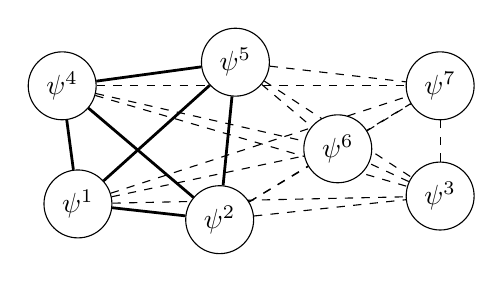
\begin{tikzpicture}[scale=1, transform shape]
	  \tikzstyle{every node} = [circle, draw, fill=white]
	  \node (1) at (0.2, 0.0) {$\psi^1$};
	  \node (2) at (2.0, -0.2) {$\psi^2$};
	  \node (5) at (4.8, 0.1) {$\psi^3$};
	  \node (4) at (0.0, 1.5) {$\psi^4$};
	  \node (3) at (2.2, 1.8) {$\psi^5$};
	  \node (6) at (3.5, 0.7) {$\psi^6$};
	  \node (7) at (4.8, 1.5) {$\psi^7$};
	  \begin{scope}[on background layer]
	  \foreach \from in {1,...,7}
	    \foreach \to in {\from,...,7}
	    \draw [dashed]  (\from) -- (\to);
	  \foreach \from in {1,...,4}
	    \foreach \to in {\from,...,4}
	    \draw [line width=1pt]  (\from) -- (\to);
	  \end{scope}
	\end{tikzpicture}
	\caption{\textbf{Illustration of the model.} Each node represents a fermion while each edge represents a connection through the Hamiltonian. Although edges imply pair-wise connections, each term in the Hamiltonian connects four at a time. For example, the solid lines represent the $J_{1245}$ term.}
	\label{fig:model}
\end{figure}

\subsection{$\cal{N}=1$ Supersymmetry}\emph{} \label{sub:N1susy}

The discussion of the supersymmetric models comes from reference~\cite{fu16}. In the $\cal N=1$ supersymmetric generalization, the Hamiltonian is written in terms of the single supercharge
\begin{align}
Q = i\sum_{i<j<k}C_{ijk}\psi^i\psi^j\psi^k,
\end{align}
where $C_{ijk}$ are now drawn from a Gaussian with mean 0 and variance $2J/N^2$. This is a $\hat{q} = 3$ model, where $\hat{q}$ is now the number of particles in each term of the supercharge. 

It might seem strange to define a supercharge when there are no bosonic operators. However, bilinear operators $\psi^i\psi^j$ behave like bosons because they do not change the fermion number. Operators $b^i$, where
\begin{align}
b^i \equiv \acom{Q}{\psi^i} = \sum_{i;j<k}C_{ijk}\psi^j\psi^k,\quad \comm{Q}{b^i}
	= \comm{H}{\psi^i} = \partial_t\psi_i, \label{eqn:N1bosons}
\end{align}
can be interpreted as the bosonic operators. Compare the above commutation and anticommutation relations with equations~\ref{eqn:repl} and~\ref{eqn:partialt}.

The Hamiltonian is defined as
\begin{align}
H &= Q^2 = - \sum_{i<j<k}C_{ijk}\psi^i\psi^j\psi^k\sum_{\l<m<n}C_{\l mn}\psi^\l
	\psi^m\psi^n.
\end{align}
Each term can contain 3, 2, 1, or 0 matching indices. For those terms where $(i,j,k) = (\l,m,n)$, the sum becomes
\begin{align}
-\sum_{i<j<k} C_{ijk}^2 \psi^i\psi^j\psi^k \psi^i\psi^j\psi^k = \th{8} 
	\sum_{i<j<k}C_{ijk}^2.
\end{align}
For any term of the form $\psi^i\psi^j\psi^k\psi^i\psi^j\psi^\l = -\th{4}\psi^k\psi^\l$, there is also a term of the form $-\th{4}\psi^\l\psi^k=\th{4}\psi^l\psi^\l$ which cancels it. Therefore there are no quadratic terms in the Hamiltonian. Terms of the form $\psi^i\psi^j\psi^m\psi^k\psi^\l\psi^m = \th{2}\psi^i\psi^j\psi^k\psi^\l$ also pair with their complements to form $\psi^k\psi^\l\psi^i\psi^j$, which in this case has the same sign as the former, leading to quartic terms
\begin{align}
-C_{ijm}C_{k\l m}\psi^i\psi^j\psi^k\psi^\l = -\th{8}C_{i[jm}C_{k\l]m} \psi^i \psi^j \psi^k\psi^\l,
\end{align}
with equality due to the antisymmetry of $C$ and the $\psi^i$. Lastly, any term with no matching $\psi$ also cancels with its complement, as in the quadratic case.

The Hamiltonian becomes
\begin{align}
H = E_0 + \sum_{i<j<k<\l}J_{ijk\l}\psi^i\psi^j\psi^k\psi^\l, \label{eqn:N1def}
\end{align}
where
\begin{align}
E_0 = \sum_{i<j<k} C_{ijk}^2\;,\qquad J_{ijk\l} = -\th{8}\sum_{a} C_{a[ij}
	C_{k\l]a}.
\end{align}
The $J_{ijk\l}$ terms connect the $N$ fermions, 4 at a time. Figure~\ref{fig:model} can also be used to represent this model.

The supersymmetry of this model is broken, because $Q$ does not in fact annihilate the vacuum due to the fermions being Majorana. Therefore there is no reason the ground state must have 0 energy. However, the ground state energy scales as $\e^{-\alpha N}$ where $\alpha$ is a constant~\cite{mald16}. The result of this is that the supersymmetry is not broken for large $N$. It is possible to keep the supersymmetry intact even for small $N$ by considering the $\cal N=2$ model.

\subsection{$\cal{N}=2$ Supersymmetry}\emph{} \label{sub:N2susy}

In $\cal N=2$ supersymmetry, two supercharges are necessary. To create these, define a new set of fermions, now complex (Dirac), that consists of $\psi^i$ and their conjugates $\psi^\dag_i$. These obey the relations 
\begin{align}
\{\psi^i,\psi^j\} = 0, \quad \{\psi^\dag_i,\psi^\dag_j\} = 0, \quad
	\{\psi^i,\psi^\dag_j\} = \delta_j^i. \label{eqn:N2_ant}
\end{align}
The supercharges, with $\hat{q}=3$ still the number of fermions per term, are
\begin{align}
Q &= i\sum_{i<j<k}C_{ijk}\psi^i\psi^j\psi^k,\quad
Q^\dag = i\sum_{i<j<k}\bar C^{ijk}\psi^\dag_i\psi^\dag_jk,
	\label{eqn:N2charge}
\end{align}
where the $C_{ijk}$ are complex numbers drawn from a 0-centered Gaussian such that
\begin{align}
\ex{C_{ijk}\bar C^{ijk}} = \frac{2J}{N^2}.
\end{align} 
The bosonic operators are defined as
\begin{align}
b^\dag_i = \acom{Q}{\psi^\dag_i} = \sum_{j<k}C_{ijk}\psi^j\psi^k,\quad 
	\comm{Q}{b_i^\dag} = \partial_t\psi_i^\dag,
\end{align}
in close analogy to equation~\ref{eqn:N1bosons}.
An analysis similar to that in the previous subsection shows the Hamiltonian $H = \acom{Q}{Q^\dag}$ can be written as
\begin{align}
H = E_0 + \sum_{ijk\l}J_{ij}^{k\l}\psi^i\psi^j\psi^\dag_k\psi^\dag_\l.
\end{align}
Like in the $\cal N=1$ case, the components of $J$ are no longer independent.
\begin{figure}
	\centering
	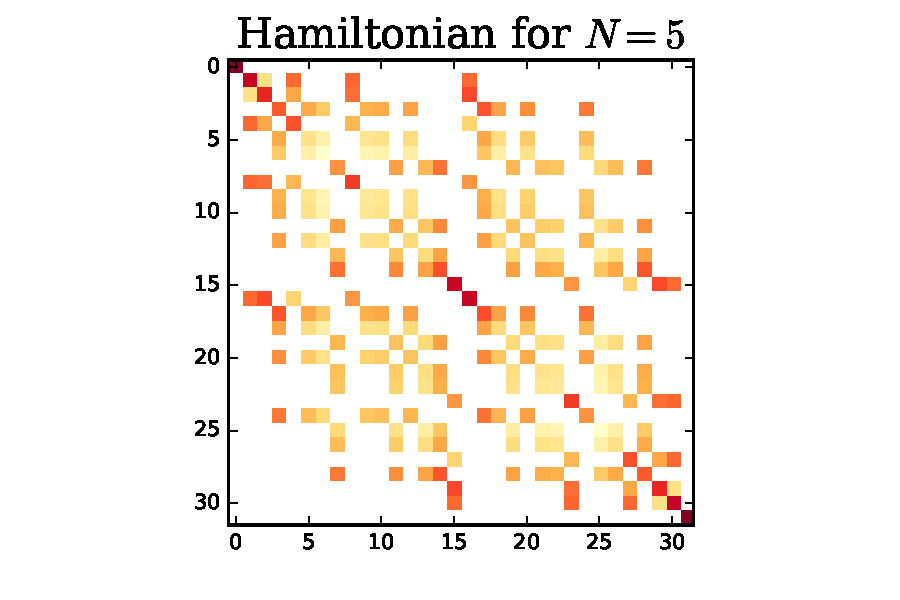
\includegraphics[width=.49\textwidth]{hamil5}
	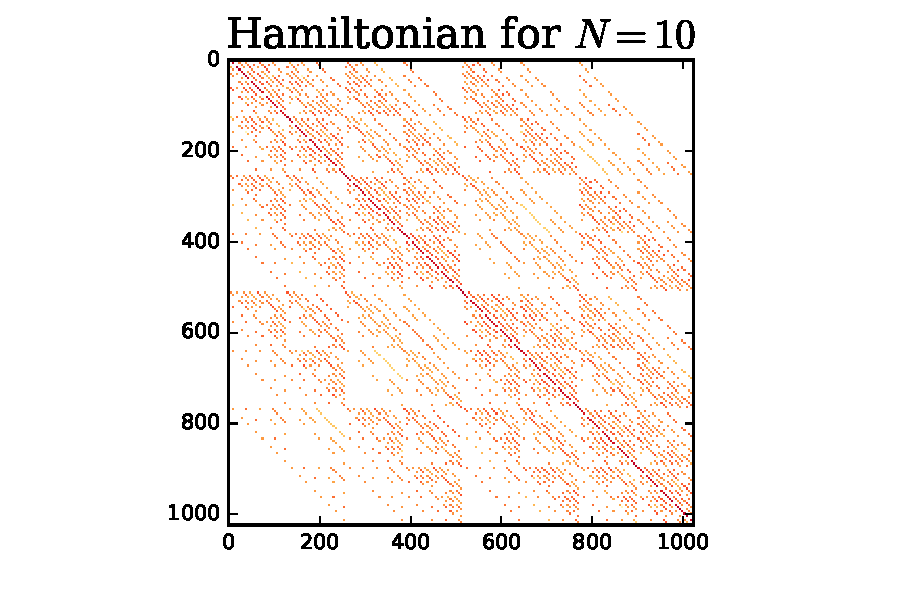
\includegraphics[width=.49\textwidth]{hamil10}
	\caption{\textbf{Plots of Hamiltonians,} where darker colors represent larger magnitude elements. For $N=5$, it is possible to see that $H$ only connects states with equal Fermi numbers. For example see the second row, corresponding to $i=1,2,4,8,16$, which each have a single `1' in their binary representations. }
	\label{fig:hamplot}
\end{figure}
Since $H$ consists of an equal number of raising and lowering operators, it preserves $F$, the Fermi number. Figure~\ref{fig:hamplot} shows this behavior.

The operators $Q^2$ and ${Q^\dag}^2$ are both 0. That implies that both $Q$ and $Q^\dag$ are conserved, as for example
\begin{align}
[H,Q] = QQ^\dag Q + Q^\dag QQ - QQQ^\dag + QQ^\dag Q = 0.
\end{align}
This also means they generate a symmetry of the Hamiltonian. This allows the methods of subsection~\ref{sub:susy} to be used to count ground states.

\section{$\cal{N}$ = 2 Ground States and Entropy} \label{sec:N2gs_ent}

The long-range order and large number of ground states in the $\cal N = 2$ supersymmetric model lead to nonzero entropy in subsystems of ground states, even at zero temperature. Calculations in this section closely follow the corresponding analysis in~\cite{fu16}.

\subsection{Counting Ground States} \emph{}\label{sub:count_gs}

A convenient way to bound the number of ground states from below is to partition the Hilbert space into energy eigenspaces with states connected by the supercharges. It will be shown that any space with an odd number of states must be made of ground states. Consider a stationary state $\ket{\phi_E}$ with energy $E$. Consider also the states $\ket{q_E} = Q\ket{\phi_E}$ and $\ket{q^\dag_E}= Q^\dag \ket{\phi_E}$. These states will have the same energy eigenvalue $E$, if they exist. 

The two simple cases are if $\ket{q}$ and/or $\ket{q^\dag}$ does not exist. If $Q$ and $Q^\dag$ both annihilate $\ket{\phi_E}$, then $E=0$. If $Q^\dag$ annihilates $\ket{\phi_E}$ but $Q$ does not, then 
\begin{align}
H\ket{\phi_E} = (QQ^\dag + Q^\dag Q)\ket{\phi_E} = Q^\dag Q\ket{\phi_E} = E\ket{\phi_E}
\end{align}
and the state $\ket{f_E} = Q^\dag Q\ket{\phi_E}$ is just $\ket{\phi_E}$, $E>0$. The same analysis applies if $Q$ annihilates but $Q^\dag$ does not. These cases are illustrated in figure~\ref{fig:tuplets1}.

\begin{figure}
	\centering 
	\begin{tikzpicture}[scale=.9, transform shape]
	\tikzstyle{every node} = [rectangle]
	\node (phi)  at (1,0) {$\ket{\phi_E}$};
	\node (q)    at (0, 2) {$Q\ket{\phi_E}$};
	\node (qbar) at (2, 2) {$Q^\dag\ket{\phi_E}$};
	\draw [->]   (phi) -- (q);
	\draw [->]   (phi) -- (qbar);
	\fill (3.5,.5) circle (1pt);
	\fill (3.5,1.5) circle (1pt);
	\node (phi)  at (6,0) {$\ket{\phi_a}$};
	\node (q)    at (5, 2) {0};
	\node (qbar) at (7, 2) {0};
	\draw [->]   (phi) -- (q);
	\draw [->]   (phi) -- (qbar);
	\node (,)    at (8.5,.5){,};
	\node (phi)  at (11,0) {$\ket{\phi_b}$};
	\node (q)    at (10, 2) {$\ket{q_b}$};
	\node (qbar) at (12, 2) {0};
	\node (E)    at (11, 4) {$\ket{f_{b}} = E_b\ket{\phi_b}$};
	\draw [->]   (phi) -- (q);
	\draw [->]   (phi) -- (qbar);
	\draw [->]   (q)-- (E);
	\end{tikzpicture}
	\caption{\textbf{Energy Eigenstate Tuplets} with either $Q$ or $Q^\dag$ annihilating the states. Arrows up and to the left and right represent the effects of $Q$ and $Q^\dag$, respectively. $\ket{\phi_a}$ must be a ground state. If $E_b\ne0$, then $\ket{f_{b}}=\ket{\phi_b}$ and the tuplet contains only two states.}
	\label{fig:tuplets1}
\end{figure}

If both $\ket{q_E}$ and $\ket{q^\dag_E}$ exist and $E>0$, then
\begin{align}
H\ket{\phi_E} = E\ket{\phi_E} = (QQ^\dag + Q^\dag Q)\ket{\phi_E} = \ket{f_E} + 
	\ket{f'_E},
\end{align}
meaning 
\begin{align}
\ket{f_E} = \alpha\ket{\phi_E} + \beta\ket{\xi_E},\qquad \ket{f'_E} = 
	(1-\alpha)\ket{\phi_E} - \beta\ket{\xi_E}.
\end{align}
$\ket{q_E}$ and $\ket{q^\dag_e}$ must be distinct, so $\ket{\xi_E}$ must exist. Therefore this tuplet also contains four states. Figure~\ref{fig:tuplets2} illustrates this case.

\begin{figure}
	\centering 
	\begin{tikzpicture}[scale=.9, transform shape]
	\tikzstyle{every node} = [rectangle]
	\node (phi)  at (1,0) {$\ket{\phi_E}$};
	\node (q)    at (0, 2) {$Q\ket{\phi_E}$};
	\node (qbar) at (2, 2) {$Q^\dag\ket{\phi_E}$};
	\draw [->]   (phi) -- (q);
	\draw [->]   (phi) -- (qbar);
	\fill (3.5,.5) circle (1pt);
	\fill (3.5,1.5) circle (1pt);
	\node (phi)  at (7, 0) {$\ket{\phi_c}$};
	\node (q)    at (5, 2) {$\ket{q_c}$};
	\node (qbar) at (9, 2) {$\ket{q^\dag_c}$};
	\node (f)    at (6, 4) {$\ket{f_c}$};
	\node (fpr)  at (8, 4) {$\ket{f_c'}$};
	\draw [->]   (phi)  -- (q);
	\draw [->]   (phi)  -- (qbar);
	\draw [->]   (q)    -- (f);
	\draw [->]   (qbar) -- (fpr);
	\end{tikzpicture}
	\caption{\textbf{Energy Eigenstate Tuplets} with neither $Q$ nor $Q^\dag$ annihilating the states. Since $\ket{f_c}$ and $\ket{f_c'}$ must be distinct (otherwise $\acom{Q}{Q^\dag}\ket{\phi_c}=Q^2\ket{\phi_c} = 0$), they each must be linear combinations of $\ket{\phi_c}$ with another state $\ket{\xi_c}$.}
	\label{fig:tuplets2}
\end{figure}

The previous analysis divides the space into tuplets of energy eigenstates with at most 4 members. All tuplets contain an even number of states, except for the ground state tuplets. All even tuplets contain an equal number of fermionic and bosonic states because the supercharges interchange bosonic states with fermionic states.

This provides the opportunity to count ground states using the Fermi number
\begin{align}
F = \sum_i\psi^\dag_i\psi^i,
\end{align}
which is even for bosonic states and odd for fermionic states. For all paired subspaces with non-zero energy, the Witten index 
\begin{align}
W = \Tr(-1)^F\label{eqn:N2witten}
\end{align}
evaluates to 0. Then the trace over the whole space has contributions only from the ground states, so the number of ground states will be equal to or greater than $|W|$. As a result, the modified Witten index $\Tr\left((-1)^F\e^{\beta H}\right)$ is independent of temperature $1/\beta$ because $H$ is zero in the ground states. 

Define the unitary operator 
\begin{align}
R^p = \e^{\frac{2\pi ipF}{\hat q}},\quad R^{\hat{q}} = \mathbb{1}.
\end{align}
$R$ commutes with $Q$ so that $\Tr\left((-1)^FR^p\right)$ also only has contributions from the ground state. This suggests a modified Witten index
\begin{align}
W_p = \Tr\left((-1)^FR^\frac{2\pi ip}{\hat q}\right).
\end{align}
Since $W$ is independent of the coupling, the Hamiltonian can be turned off, in which case the index is just the product of the indexes over all particles $\left(Z^{(1)}\right)^N$ so that 
\begin{align}
W_p = \left(1-\e^{\frac{2\pi ip}{\hat{q}}}\right)^N = e^{i\pi N\left(\frac{p}{\hat q} - \th{2}\right)}\left(2\sin\frac{\pi p}{\hat q}\right)^N
\end{align}
and the degeneracy of the ground state is 
\begin{align}
D_\text{GS} \ge \abs{W} = \left(2\sin\frac{\pi p}{\hat q}\right)^N. \label{eqn:dgs}
\end{align}
To provide the highest bound on $D_\text{GS}$, choose $p = (\hat q+1)/2$, so that $D_\text{GS} \ge \sqrt{3}^N$, where $\hat q = 3$ for the supercharge in equation~\ref{eqn:N2charge}.

Compare this to the total number of states $2^N$. It is clear that the number of ground states is extensive, as the number of degrees of freedom, the logarithm of $D_\text{GS}$, scales linearly with $N$.

\subsection{Ground State Entanglement Entropy} \emph{} \label{sub:entangle}

The large number of ground states has an interesting effect on the entanglement entropy of a subsystem of a ground state. Classically, entropy $\cal H = -\sum_ip_i\log p_i$ measures uncertainty about an event, where $p_i$ are the probabilities of distinct outcomes. $\cal H$ ranges from 0 for events in which the outcome is known, to $\log m$ if there are $m$ possibilities with equal probabilities. 

The nearest quantum mechanical analogue is Von Neumann entropy
\begin{align}
S = -\Tr(\rho\log\rho).\label{eqn:vnent}
\end{align}
In the eigenbasis of $\rho$, where $\rho = \sum_i p_i\ket{i}\bra{i}$,
\begin{align}
S = -\sum_{ij}\braket{j}{i}p_i\braket{i}{j} = -\sum_ip_i\log p_i,
\end{align}
which mimics the classical form.

The entropy of a pure state is always 0. However, subsystems of a pure state are mixed, and therefore have non-zero entropy. This entropy does not represent uncertainty, since the state of the whole system is known. Rather, it represents the classical mutual information between the two subsystems, or the maximum amount of information that can be gained about one by local measurements on the other, without classical information transfer~\cite{janzing09}. This suggests an analogy with black holes, as information cannot classically pass an event horizon~\cite{ryu06}.

\begin{figure}
	\centering
	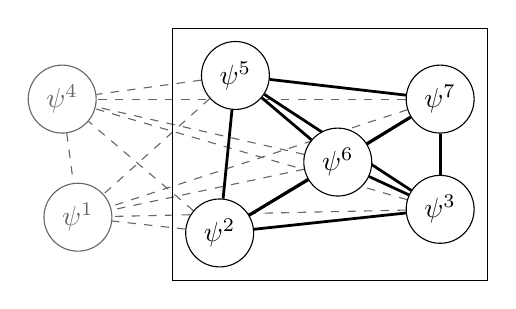
\begin{tikzpicture}
	  \tikzstyle{every node} = [circle, draw=mygray, fill=white]
	  \node (7) at (0.2, 0.0) {\textcolor{mygray}{$\psi^1$}};
	  \node (5)[draw=black] at (2.0, -0.2) {{$\psi^2$}};
  	  \node (1)[draw=black] at (4.8, 0.1) {$\psi^3$};
  	  \node (6) at (0.0, 1.5) {\textcolor{mygray}{$\psi^4$}};
	  \node (4)[draw=black] at (2.2, 1.8) {{$\psi^5$}};
	  \node (2)[draw=black] at (3.5, 0.7) {$\psi^6$};
	  \node (3)[draw=black] at (4.8, 1.5) {$\psi^7$};
	  \begin{scope}[on background layer]
	  \foreach \from in {1,...,7}
	    \foreach \to in {\from,...,7}
	    \draw [dashed, color=mygray]  (\from) -- (\to);
	  \foreach \from in {1,...,5}
	    \foreach \to in {\from,...,5}
	    \draw [line width=1pt]  (\from) -- (\to);
	  \end{scope}
	  \draw (1.4, -.8) rectangle (5.4, 2.4);
	\end{tikzpicture}
	\caption{\textbf{Subsystem of the Model.} If fermions 1 and 4 are traced out, the resulting density matrix describes the relationships between the others.}
	\label{fig:subsys}
\end{figure}

Consider state $\ket{\phi}_\cal{A}$ on a system $\cal A$ that can be decomposed into subsystems $A$ and $B$. The state can in general be written as 
\begin{align}
\ket{\phi}_\cal{A} = \sum_jc_j\ket{\phi_j}_A\ket{\phi_j}_B,
\end{align}
where the $\ket{\phi_j}$ are orthogonal in each subsystem. Then $j$ can only run over the dimension $m$ of the smaller subspace. Since the reduced density matrices $\rho_A = \Tr_B\rho_{\cal A}$ are
\begin{align}
\rho_A = \sum_jp_j\ket{\phi_j}_A\bra{\phi_j}_A, \quad \rho_B = \sum_jp_j\ket{\phi_j}_B\bra{\phi_j}_B; \quad p_j = |c_j|^2,
\end{align}
it is clear that the entropies of entanglement are equal for each subsystem. In fact, they satisfy 
\begin{align}
S(\rho) = S(\rho_B) = \cal{H}(p_j),
\end{align}
where $\cal H$ is the classical entropy with $p_j$ interpreted as classical probabilities. 

A general ground state in the $\cal N=2$ SYK model can be written as 
\begin{align}
\ket{\phi_0} = \sum_ic_i\ket{i}_A\ket{i}_B. \label{eqn:mixed}
\end{align}
If the smaller of the two subsystems has $m$ dimensions, the sum in~\ref{eqn:mixed} can contain at most $2^m$ terms, the maximum number of states in the smaller subsystem. Maximum entropy is achieved when the coefficients $c_i$ are equal, so 
\begin{align}
S_\text{max} = \sum_{i=1}^{2^m}\th{2^m}\log 2^m = m\log(2).\label{eqn:thermal}
\end{align}
This is a general bound on the bipartite entanglement entropy of any system.

Another type of entropy is the ground state entropy, defined as $S_\text{GS} = \log D_\text{GS}$. To understand the connection to entanglement entropy, consider a system entangled with its environment. If the system is known to be in a ground state, the maximum entanglement entropy possible is $S_\text{max} = \log D_\text{GS} = S_\text{GS}$.

\section{Numerical Results} \label{sec:numeric}

Computations on the $\cal N=2$ model were completed in Python using Numpy~\cite{vander11}. Except for the $N=12$ models, all were run on a laptop.

\subsection{Building Matrices}\emph{} \label{sub:build_mat}

The simplest way to compute large-N functions on a computer is to use a matrix representation for the group. This can be done by viewing the $\psi^\dag$ and $\psi$ operators as raising and lowering operators, respectively. Consider the case of $N$ fermions. Write the state as an $N$-dimensional binary vector
\begin{align}
\ket{m} = \ket{m_1m_2\dots m_i\dots m_{N-1}m_N}, \quad\sum_im_i2^{i-1} =
	m.\label{eqn:2Nstate}
\end{align}
The vacuum state is $\ket{0}$. A populated state can be written as
\begin{align}
\ket{110\dots 0} = \psi^\dag_1\psi^\dag_2 \ket{0} =-\psi^\dag_2\psi^\dag_1\ket{0},
\end{align}
which enforces the canonical ordering through anticommutation relations. 

The matrix representations of $\psi^i, \psi^\dag_i$ are then calculated component-wise as a $2^N$ by $2^N$ matrix.
\begin{align}
\psi^\dag_i &= \sum_{a,b}\ket{a}\psi^\dag_{i,ab}\bra{b}\nn
\psi^\dag_{i,ab} &= \brakett{a}{\psi^\dag_i}{b}.\label{eqn:comps}
\end{align}
These components may be calculated effectively using the pseudocode in figure~\ref{code:psibar}.

\begin{figure}[ht]
	\begin{lstlisting}[language=python][gobble=2]
    def psi_bar(N,i):
      psi_bar = np.zeros((2^N,2^N))
      for (n,m) in psi_bar:
        if (m-n == 2^j) and (n & 2^j == 0): 
          psi[m,n] = (-1)^Fermi(n,j),
    return psi_bar
	\end{lstlisting}
	\cprotect\caption{\textbf{Code for generating $\psi^\dag$ matrices,} where \verb|^| represents exponentiation, \verb|&| represents bitwise and \verb|Fermi(n,j)|, the reduced Fermi number, is the number of nonzero components in \verb|n| before the \verb|j|'th component. This handles anticommutation requirements. A similar structure can be used for building the $\psi$ matrices.}
	\label{code:psibar}
\end{figure}

It is also possible to create the matrices recursively. The base case is $N=1$, for which the matrices are the raising and lowering matrices,
\begin{align}
\psi^\dag_{1,(1)} = \begin{bmatrix} 0&0\\1&0 \end{bmatrix}, \qquad
    \psi^1_{(1)} = \begin{bmatrix} 0&1\\0&0 \end{bmatrix}. \label{eqn:base}
\end{align}
Then, to increase the dimension take the tensor product with the $2\times 2$ identity matrix $I$,
\begin{align}
\psi^\dag_{i,(N)} = I\otimes\psi^\dag_{i,(N-1)},\quad \psi^i_{(N)} = I\otimes 
	\psi^i_{(N-1)}.
\end{align}
This formula of course does not work when $i=N$. In this case the solution is still to use recursion, with the formula
\begin{align}
\psi^\dag_{i,(N)} = \psi^\dag_{i-1,(N-1)}\otimes\sigma_3,
\end{align}
with equation~\ref{eqn:base} again supplying the base case.

Although there are various representations of the group, the previous two constructions lead to the same representation. The analysis in this paper used the former method because of its relative simplicity.

\subsection{Ground States} \emph{} \label{sub:num_gs}

Counting ground states was implemented by counting the zero eigenvalues of a randomly-generated Hamiltonian. The number of ground states stayed above the bound in equation~\ref{eqn:dgs}, although the bound was not tight in some places. See figure~\ref{fig:gserr} for the number of ground states above the bound.

\begin{figure}
	\centering
	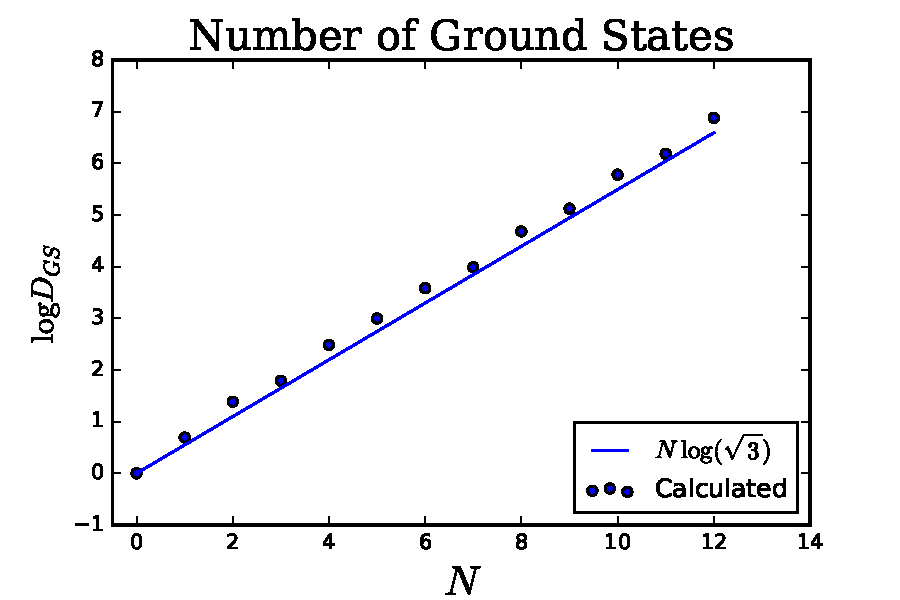
\includegraphics[width=.49\textwidth]{gscount}
	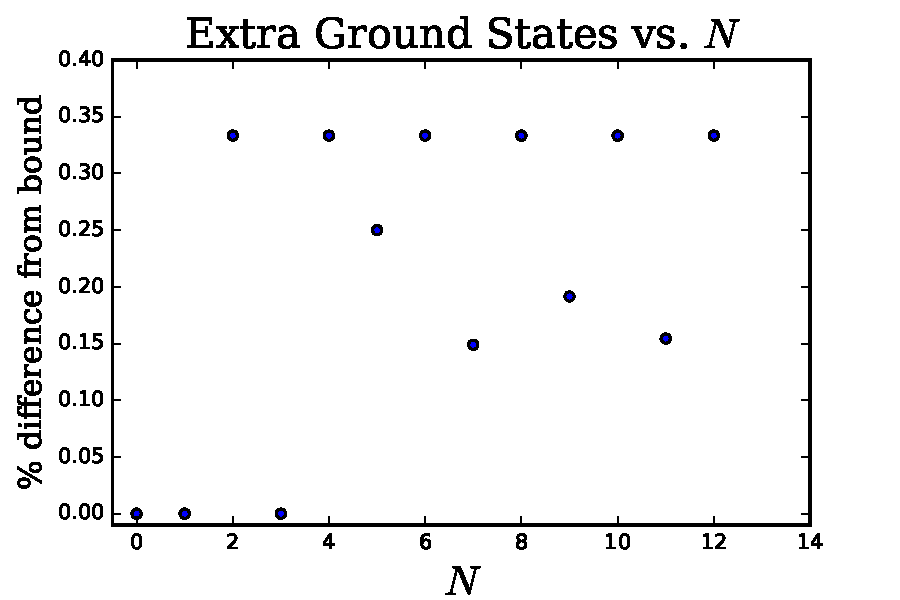
\includegraphics[width=.49\textwidth]{gserr}
	\caption{\textbf{Tightness of bound on number of ground states.} The plot on the left shows the degeneracy of the ground states calculated numerically, along with the bound $D_\text{GS} \ge \sqrt{3}^N$. The right plot shows the looseness of the bound, where 0 represents the bound being tight while 1 would mean twice as many ground states as the bound. Since the number of ground states is an integer, these values were calculated as $\text{ceil}(\sqrt{3}^N)$.}
	\label{fig:gserr}
\end{figure}

It is interesting to note that the number of ground states is particularly high for even $N$. Even with randomly generated Hamiltonians, the relative number of ground states above the bound stays about constant near 0.33 in this case.

\subsection{Ground State Entanglement Entropy}\emph{} \label{sub:num_ent}

Once the ground states were calculated for a single Hamiltonian, the entropy of a subsystem of the ground state could be calculated from the reduced density matrix of the subsystem. Starting with a ground state $\ket{\phi}$, the density matrix $\rho = \ket{\phi}\bra{\phi}$ can be calculated. Then the reduced density matrix $\rho_M$ is $\rho$ traced over $M$ particles. The entropy of the $N-M$ dimensional subsystem $S_M = -\Tr\rho_M\log\rho_M$ can be calculated as 
\begin{align}
S_M = -\sum _ip_{M,i}\log p_{M,i},
\end{align}
where $p_{M,i}$ are the eigenvalues of $\rho_M$. 

As predicted, the entropy initially rises and then drops linearly as more particles are traced over. Since the ground states depend on the random coupling, it is necessary to perform multiple calculations and average the entropies. 

Figure~\ref{fig:allentropy} shows entropy of the reduced density matrices for $N = 1,2,3...12$. The solid line shows the entropy of a thermal state as defined in equation~\ref{eqn:thermal}. When one partition is smaller than the other, the $m\log2$ bound is close to tight. 

\begin{figure}
	\centering
	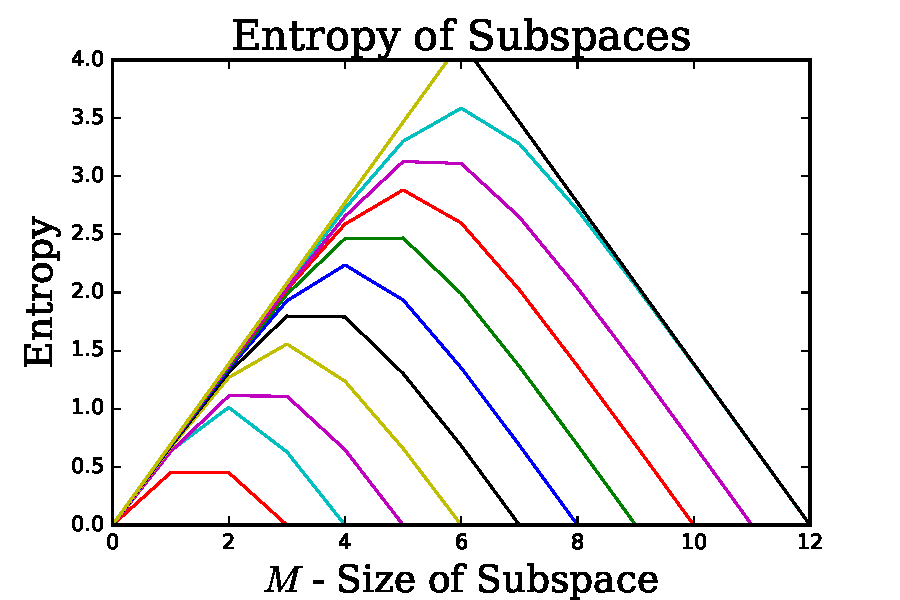
\includegraphics[width=.49\textwidth]{allentropy}
	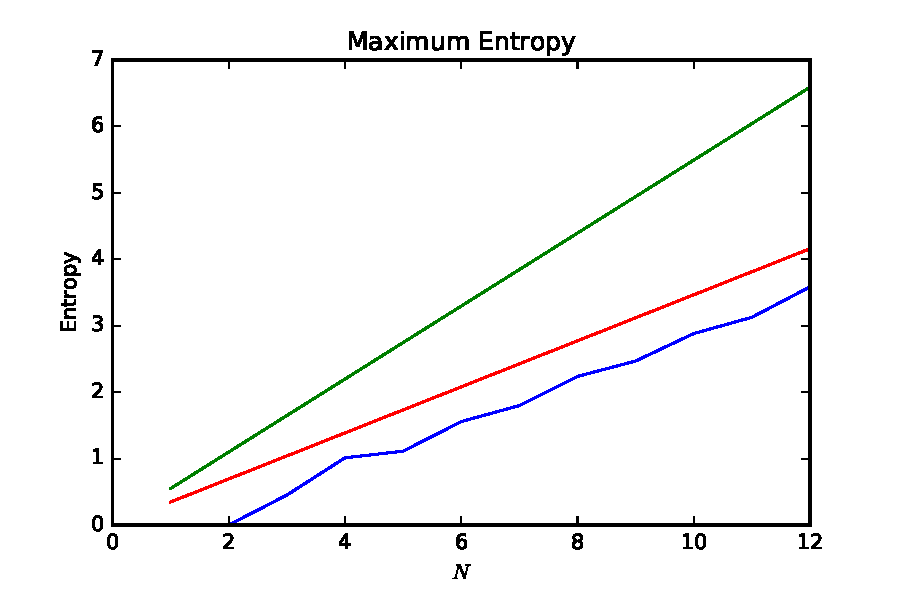
\includegraphics[width= .49\textwidth]{maxentropy}
	\caption{\textbf{Entanglement Entropy.} On the left, each curve shows the entropy for a given $N$, after tracing over $M$ particles. The straight line bounds the entropy as $m\log2$, $m = \min(M,N-M)$. The right plot shows the maximum entropy achieved for $0<N\le12$, along with the bound $N\log\sqrt{2}$.}
	\label{fig:allentropy}
\end{figure}

Close to equipartition, the entropy is smaller. Figure~\ref{fig:allentropy} also shows the maximum entropy as a function of $N$. Since maximum entropy occurs when $m = M = N/2$, this maximum value is bounded by $S_\text{max} \le N\log\sqrt{2}$.

\section{Conclusion} \label{sec:concl}

This paper introduced and discussed the supersymmetric SYK model, by first presenting supersymmetry and the SYK model separately, then the supersymmetric generalizations of the model from~\cite{fu16}. It confirmed calculations that both the ground state degeneracy and entropy are extensive, scaling with the number of particles. 

The number of ground states is consistently above the bound $\sqrt{3}^N$. In fact, for even $N$ the bound is exceeded by about $1/3$ consistently for $N<13$. These extra states presumably come from some added symmetry introduced at even $N$. Study of the source of this symmetry could be an interesting future path. 

At small $M$, the entanglement entropy is nearly maximal for a general ground state. This is not surprising, although the number of ground states could have implied a smaller upper bound on the entanglement entropy. 

Interesting future work for this project could include running similar calculations for the $\cal N=1$ model and running the calculations for higher $N$. The $\cal N=1$ calculations would not be very different to set up, but would have different results because of the difference in the theories, especially due to the broken supersymmetry at small $N$. Calculations for larger $N$ could be made efficient by exploring alternative ways to create the $\psi$ matrices, or writing the code in a faster language.

Another aspect to explore is the holographic dual of these results. The large ground state entropy and entanglement entropy should translate to large entropy in the AdS black hole.

\section*{Acknowledgments}

I would like to thank Prof. Herman Verlinde for his patience and guidance throughout the semester. Thank you also to Jaewon Kim for his help with understand the model and how to create the $\psi$ matrices.

\printbibliography

\end{document}
